\section{Examples of Human Qualitative Responses Favoring \texttt{Basic} Sampling Over \texttt{Min-P} Sampling}
\label{app:sec:human_qual_responses}

In Section~\ref{sec:human_evals:subsec:human_feedback}, we described how qualitative responses from many human participants in the original paper's study favored \texttt{basic} sampling. Direct quotes from human evaluators favoring \texttt{basic} sampling are provided below. In the study, \texttt{basic} sampling was called “Model A”; for clarity, we substituted the pseudonyms for the actual sampling methods):
%
\begin{itemize}
    \item ``[\texttt{basic} sampling] on Temp 3.0 - High Diversity setting. The stories where [sic] more interenting [sic], felt more different compared to the others, which felt like the same ideia [sic] just in a different format.”
    \item ``I felt like [\texttt{basic} sampling] was most diverse and most interesting with it's [sic] descriptions of the characters and the setting. It appealed to me most and seemed to have less 'broken' sentences that didn't make sense. Descriptions were painterly [sic] and elaborate.”
    \item ``[\texttt{basic} sampling] was more engaging, it aroused my curiosity.”
    \item ``[\texttt{basic} sampling] provided more depth and easy to read for me and there was more diversity.”
    \item ``[\texttt{basic} sampling], they presented creative storytelling”
    \item ``[\texttt{basic} sampling]. From the very beginning the verbiage and descriptions were very creative and vivid. And each story was unique”
    \item ``I believe that [\texttt{basic} sampling] has provided stories with more differentiation overall than the other two models. From the point of view of creativity, all three models are more or less equivalent as they almost always talk about stories set in extraterrestrial worlds both from a physical and mental (dreams) point of view''
    \item ``[\texttt{Basic} sampling]: Sample 2: Temperature Setting F (Temp 3.0 - High Diversity). The story was captivating, it took inside the mystical land and walked you right besides all the characters, you can even draw the characters from just th descriptions provided by the prompt. you Could even smell them, smell the setting and be at one with the setting.''
    \item ``I personally preferred [\texttt{basic} sampling] on the setting of creative, descriptive storytelling. I enjoyed how the writing was creative, showing imagination and a strong use of language. The stories were quite evocative, with intriguing settings and characters that helped to draw the reader in. I also appreciated the diversity of themes that were explored, from night weavers to dream manipulation and mysterious libraries, which kept the stories engaging and interesting.''
    \item ``Temporature setting C on [\texttt{basic} sampling] was the best. The story was fascinating and very engaging. I wanted to read more.''
    \item ``I prefered the first [\texttt{basic} sampling]. Tho [\texttt{basic} sampling] and C seem to be very head to head. But something about [\texttt{basic} sampling] seemed different in quality about it to me.''
\end{itemize}

More quotes are in the \href{https://github.com/menhguin/minp_paper/blob/main/min_p%20user%20preference%20study%20v2.0%20(Responses)%20-%20Form%20responses%201%20(1)%20(2).csv)}{original paper's data}. We urge readers to draw their own conclusions.


\clearpage
\section{GSM8K Chain-of-Thought Scores with ``Standard'' Formatting}
\label{app:sec:gsm_cot_scores}

At the request of \citet{nguyen2024minp}, we reran our GSM8K Chain-of-Thought sweeps using ``standard'' formatting instead of ``Llama'' formatting. \textbf{Both analyses reached consistent results: \texttt{min-p} does not consistently outperform other samplers when controlling the volume of hyperparameter space.}

\begin{figure}[b!]
    \centering
    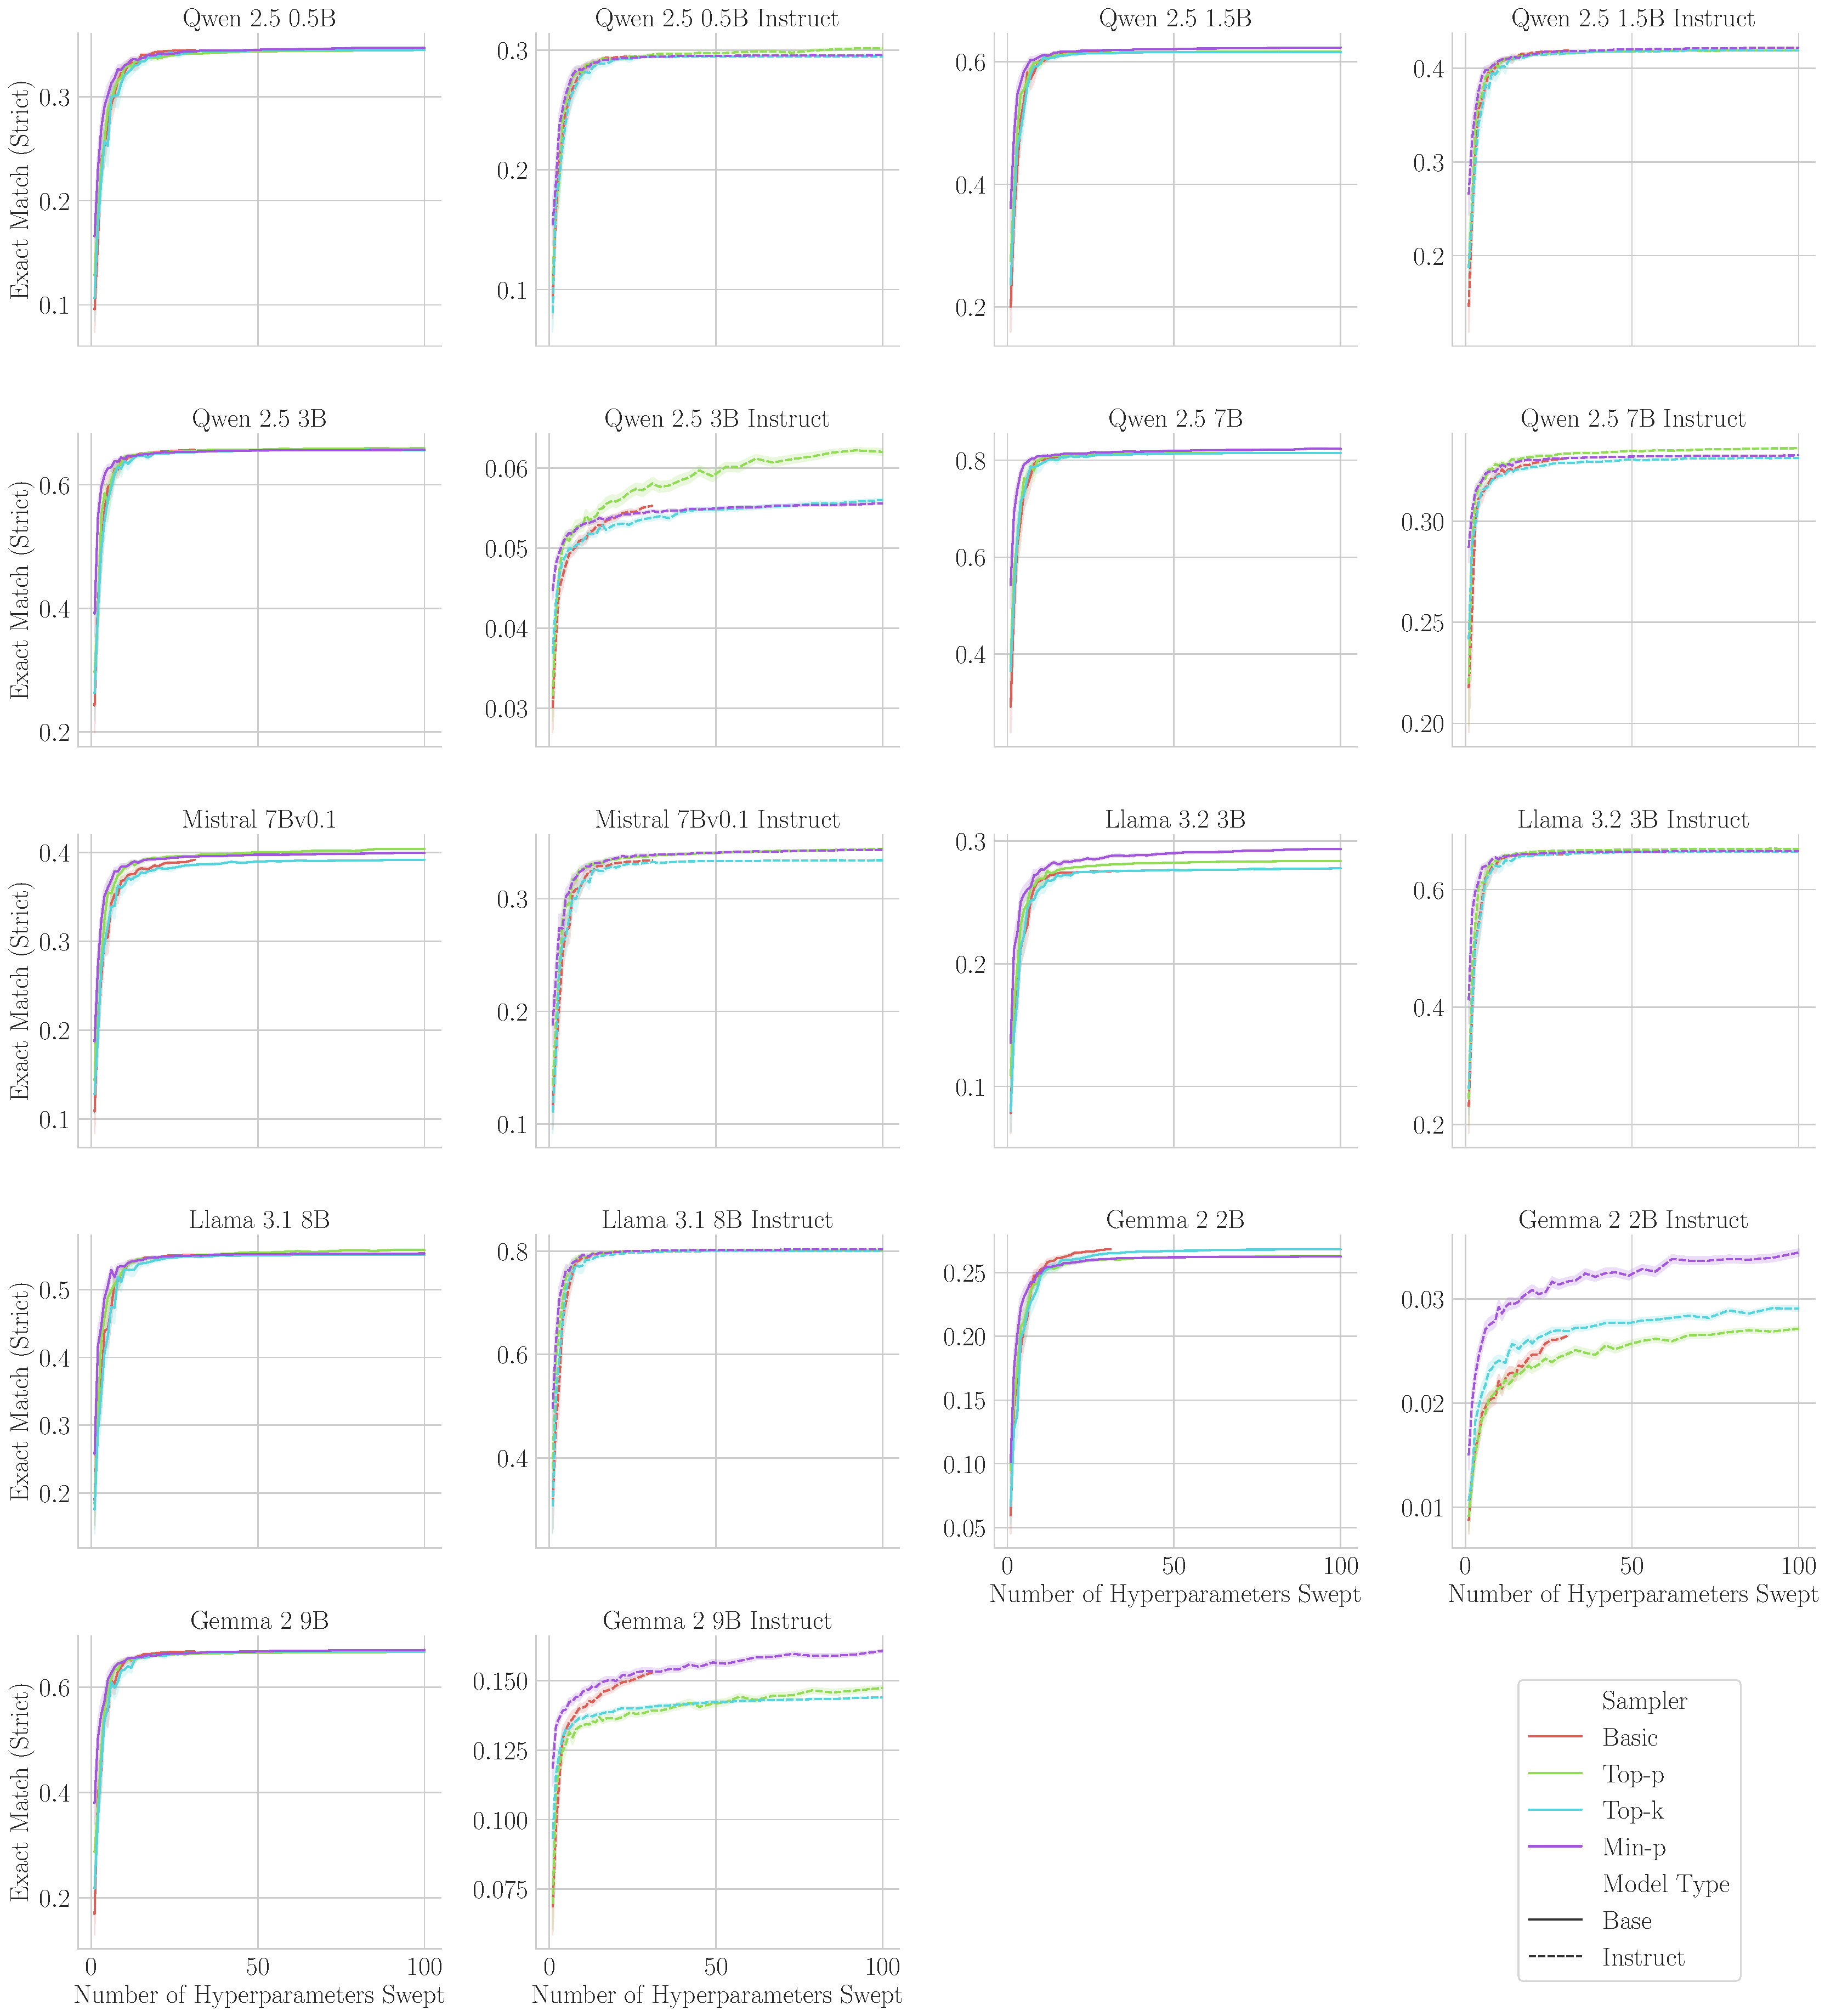
\includegraphics[width=1.0\linewidth]{figures/nlp_benchmark_evals/gsm8k_cot/y=em_strict_x=N_hue=sampler_row=model_col=task.pdf}
    \caption{\textbf{\texttt{Min-P} Does Not Consistently Outperform Other Samplers on GSM8K When Controlling For Hyperparameter Volume.}
    We reran our GSM8K sweep using ``standard'' formatting rather than ``Llama'' formatting and observed qualitatively similar data.
    }
\end{figure}

\clearpage

\begin{figure}[t!]
    \centering
    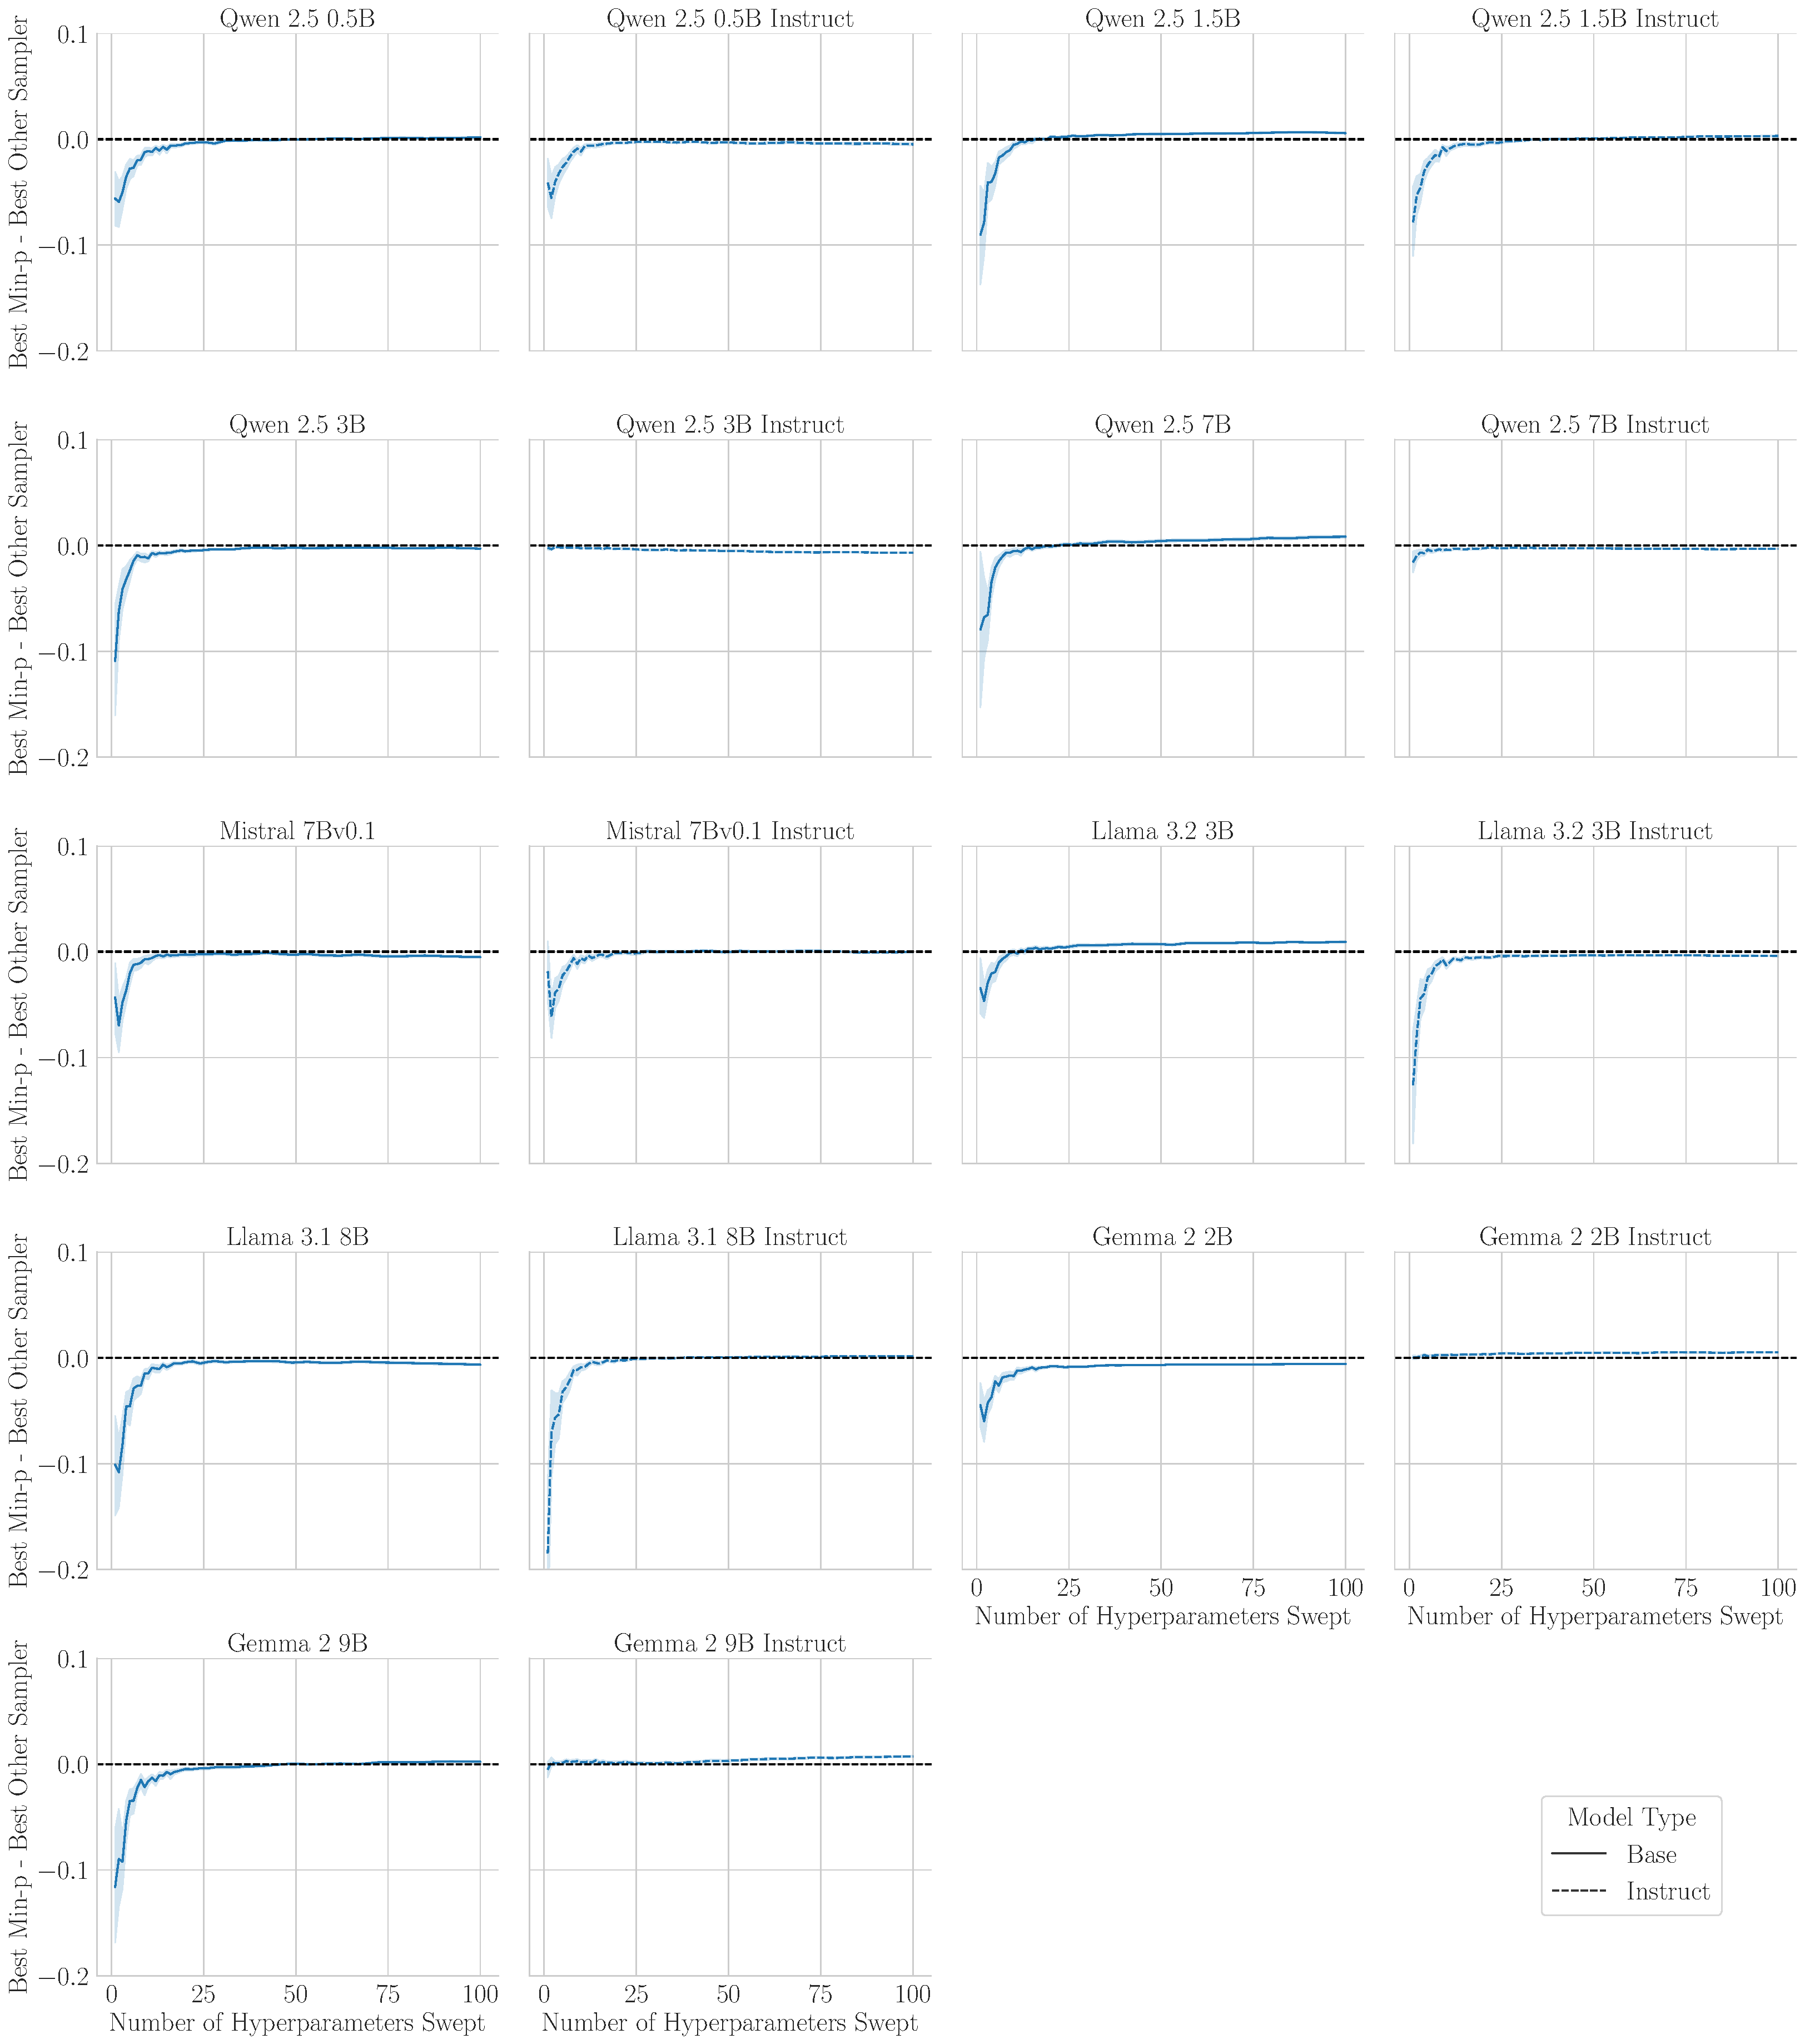
\includegraphics[width=1.0\linewidth]{figures/nlp_benchmark_evals/gsm8k_cot/y=diff_of_em_strict_x=N_hue=sampler_row=model_col=task.pdf}
    \caption{\textbf{\texttt{Min-P} Does Not Consistently Outperform Other Samplers on GSM8K When Controlling For Hyperparameter Volume.}
    We reran our GSM8K sweep using ``standard'' formatting rather than ``Llama'' formatting and observed qualitatively similar data.}
\end{figure}

\clearpage

\section{GPQA Best-of-$N$ Scores}
\label{app:sec:gpqa_scores}

\begin{figure}[h!]
    \centering
    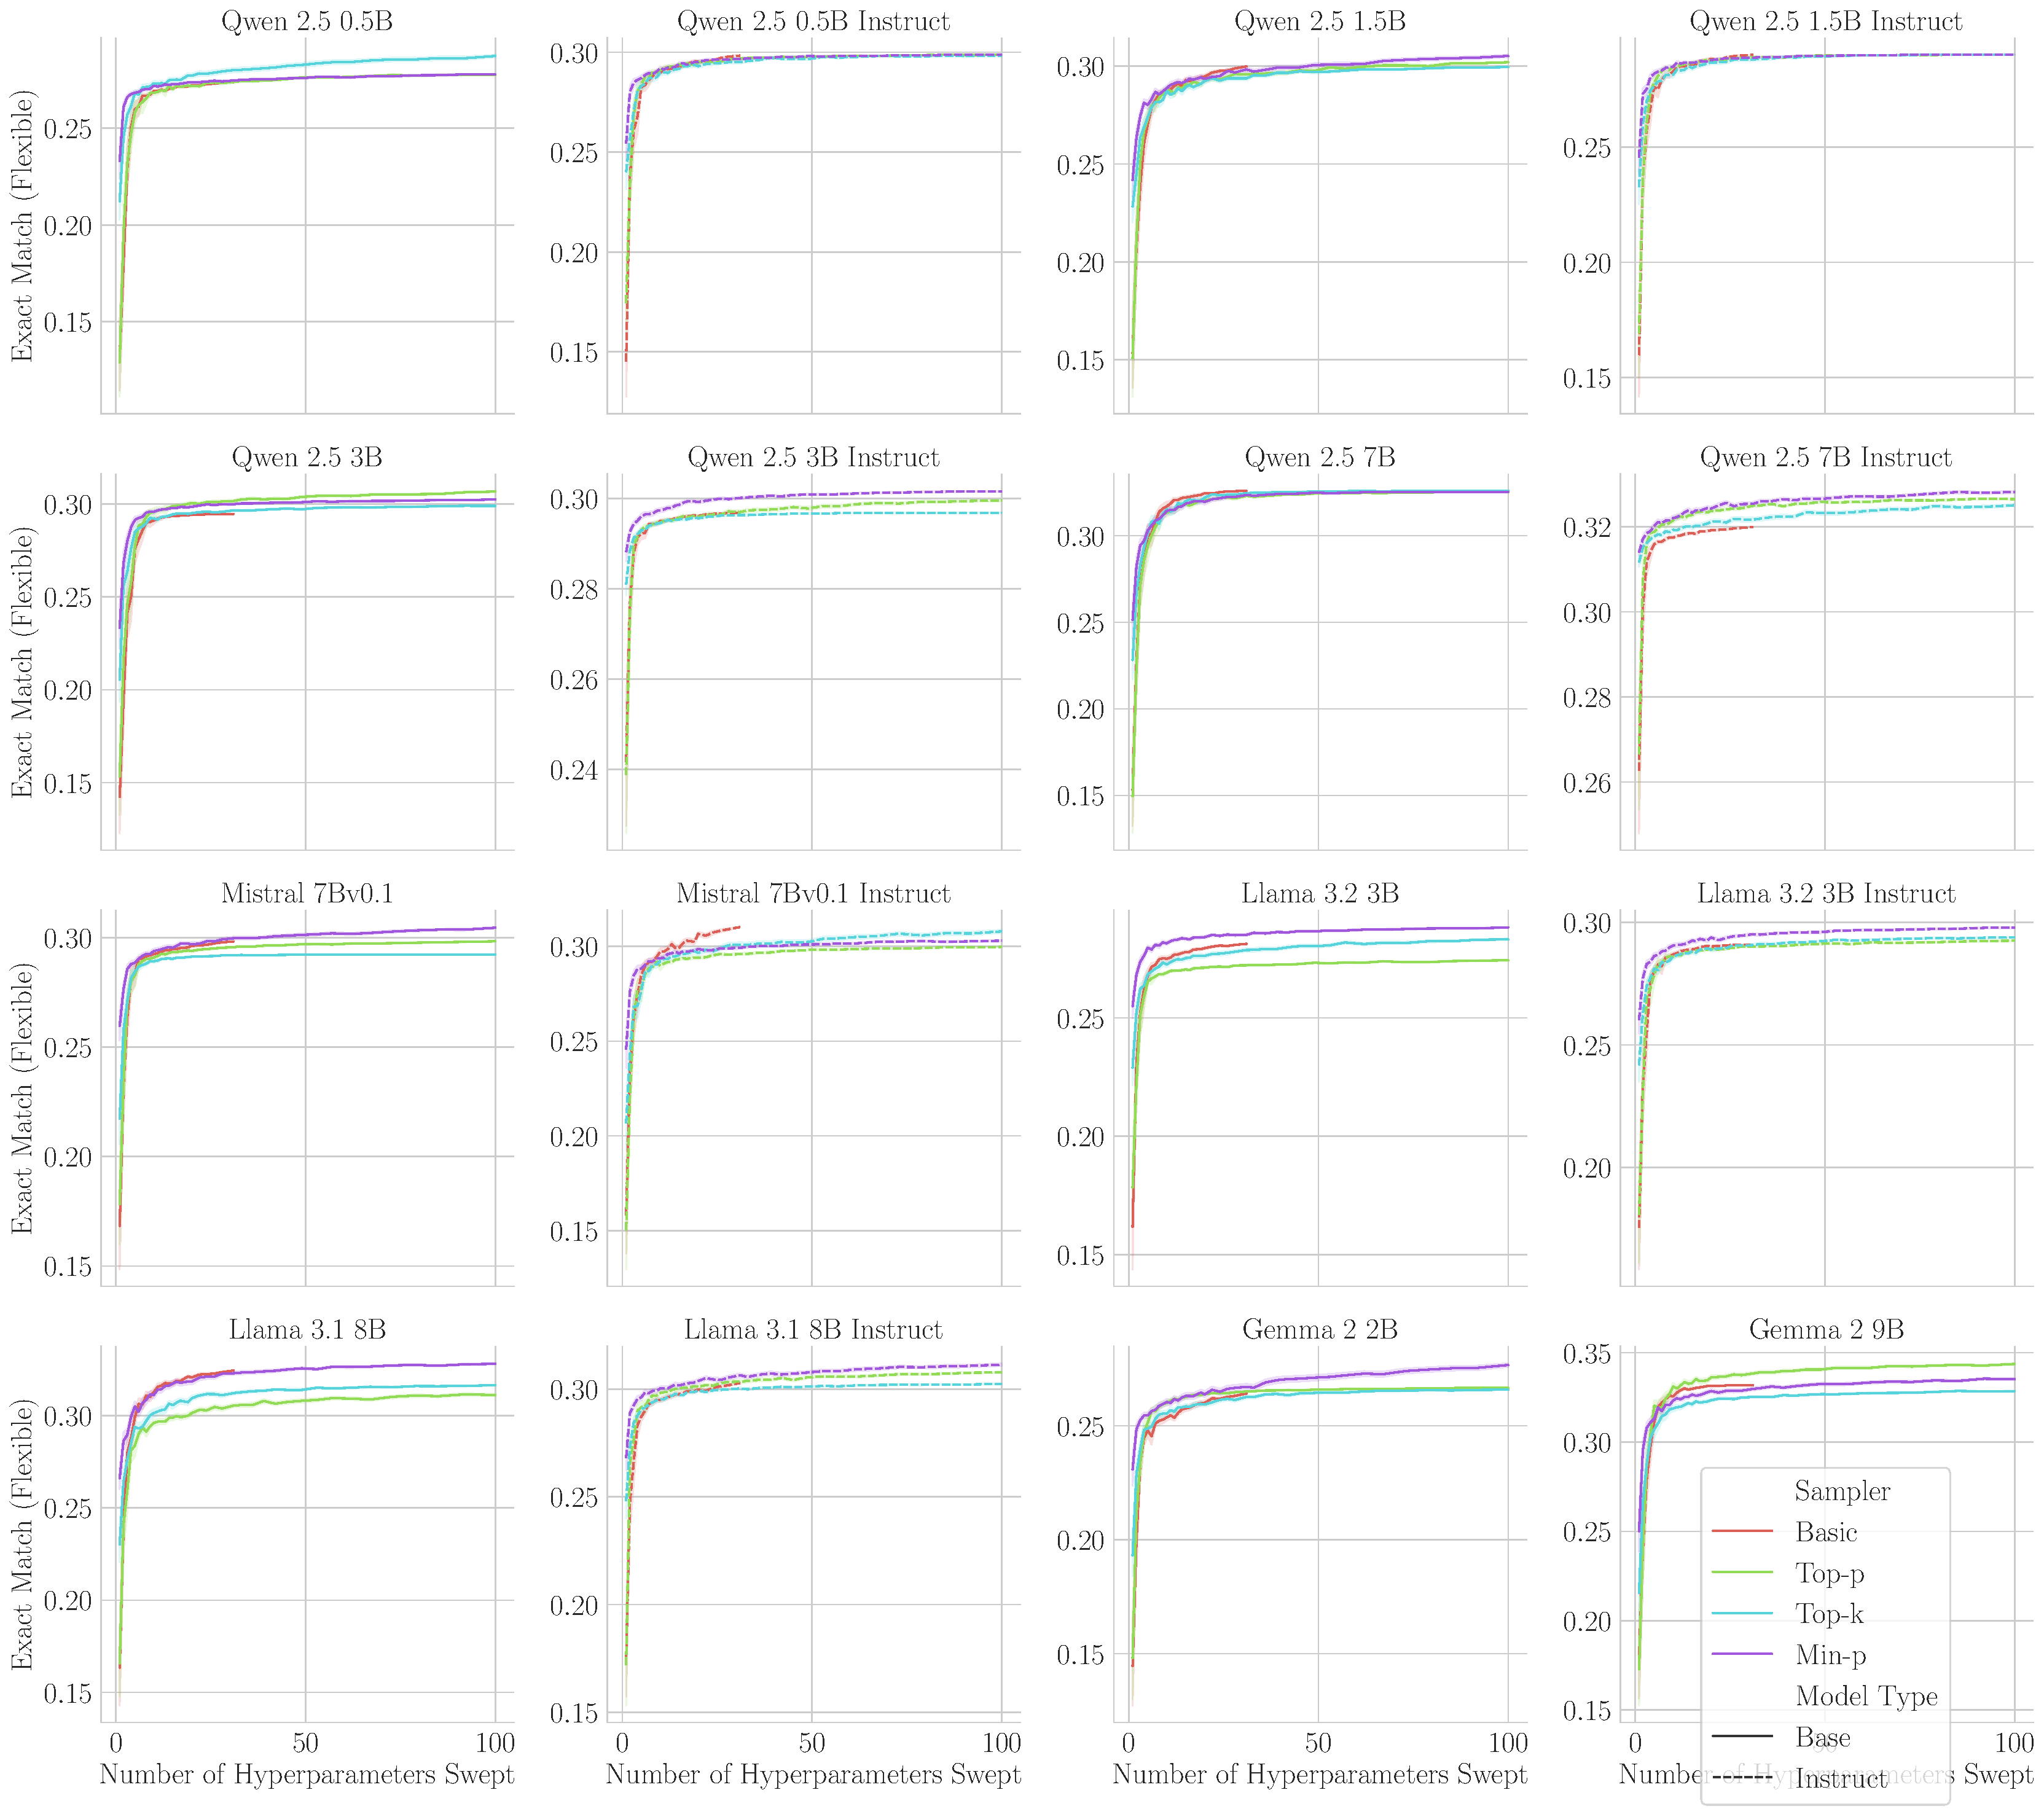
\includegraphics[width=0.8\linewidth]{figures/nlp_benchmark_evals/gpqa/y=em_flexible_x=N_hue=sampler_row=model_col=task.pdf}
    \caption{\textbf{Best-of-$N$ GPQA Scores Per Sampler.} Companion to Fig.~\ref{fig:gpqa_diff_of_em}: the best-of-$N$ flexible-extract exact match of each sampler on GPQA (5-shot) for the 16 models with complete sweeps. All four samplers reach similar scores once given the same number of hyperparameter configurations.}
    \label{fig:gpqa_em}
\end{figure}

\clearpage

\section{GSM8K Chain-of-Thought Scores on Larger Models}
\label{app:sec:gsm8k_large_models}

To partially address whether our conclusions hold for larger models, we ran the GSM8K CoT sweep of Sec.~\ref{sec:nlp_evals:subsec:gsm8k} (standard formatting) on ten additional models: Qwen 2.5 14B, 32B and 72B, Gemma 2 27B, and Llama 3.1 70B, each in base and instruct variants.
Fig.~\ref{fig:gsm8k_large_models_diff_of_em} shows the difference between the best-of-$N$ score of \texttt{min-p} and that of the best other sampler.
The conclusion is unchanged: \texttt{min-p} does not outperform other samplers when controlling for hyperparameter volume.

\begin{figure}[h!]
    \centering
    
\includegraphics[width=0.8\linewidth]{figures/nlp_benchmark_evals/gsm8k_cot_large_models/y=diff_of_em_strict_x=N_hue=sampler_row=model_col=task.pdf}
    \caption{\textbf{\texttt{Min-P} Does Not Consistently Outperform Other Samplers on GSM8K CoT for Larger Models.} Difference between the best-of-$N$ strict-match exact match of \texttt{min-p} and that of the best other sampler on GSM8K CoT (standard formatting) for ten models from 14B to 72B parameters.}
    \label{fig:gsm8k_large_models_diff_of_em}
\end{figure}

\begin{figure}[h!]
    \centering
    
\includegraphics[width=0.8\linewidth]{figures/nlp_benchmark_evals/gsm8k_cot_large_models/y=em_strict_x=N_hue=sampler_row=model_col=task.pdf}
    \caption{\textbf{Best-of-$N$ GSM8K CoT Scores Per Sampler for Larger Models.} Companion to Fig.~\ref{fig:gsm8k_large_models_diff_of_em}.}
    \label{fig:gsm8k_large_models_em}
\end{figure}

\clearpage

\section{The ICLR 2025 Review Record}
\label{app:sec:review_record}

For completeness, we note how the issues documented in the main text relate to the public ICLR 2025 review record for \citet{nguyen2024minp}.
The community adoption figures that were later retracted (Sec.~\ref{sec:community_adoption}) were cited as evidence of impact in the meta-review: the \href{https://openreview.net/forum?id=FBkpCyujtS&noteId=WH4Y2gZs6R}{Area Chair wrote} that \texttt{min-p} ``is simple and is already widely adopted by the community (as mentioned by [Reviewer] D38H, `The usage of it in 54,000 Github repositories alone is very impressive')'', and \href{https://openreview.net/forum?id=FBkpCyujtS&noteId=tMSeNlMmSa}{Reviewer fwNb wrote} that \texttt{min-p} ``has good empirical results, both as measured on benchmarks and (more important [sic]) by adoption of the community''.
The public reviews do not discuss which model(s) were sampled from in the LLM-as-a-judge evaluations or the absence of uncertainty estimates for the reported win rates (Sec.~\ref{sec:llm_as_judge_evals}).
Separately, the meta-review attributes \texttt{min-p}'s advantage to the low temperature regime (``in the low temperature regime, [\texttt{min-p}] provides a significant advantage''), whereas the paper's claims concern the high temperature regime.

\clearpage

% \section{Minor Discoveries}
% \label{app:sec:minor_discoveries}

% In this section, we compile a list of other discoveries and oddities.

% \paragraph{Human Judgments of Diversity Don't Increase with Temperature}

% As a minor comment, we note that higher temperature $\tau$ does not correspond to higher diversity scores.
% We do not know whether the human evaluations were inadequate or underpowered, or perhaps the field's conceptual understandings of temperature at the per-token level is disconnected from temperature at the sentence and paragraph level.

% \paragraph{\texttt{Min-p} Typically Scores Highest on GSM8K at Low Temperatures}

% Our GSM8K and GSM8K Llama experiments revealed a different pattern than reported by \citet{nguyen2024minp}.
% Specifically, the authors wrote:
% “Notably, across all experiments, best scores were achieved with \texttt{min-p} across a range of temperatures, rather than greedy decoding, challenging assumptions that greedy decoding is strictly optimal for task benchmarks
% \citep{castel2022optimalgreedydecodingextractive, wiher2022decoding})."
% In contrast, our more extensive sweep showed that when using \texttt{min-p}, most models achieved their best performance at low temperatures (Appendix Fig.~\ref{fig:gsm8k_per_sampler_scores}), which aligns with conventional understanding of task benchmark optimization.


% \paragraph{Swapped Column Labels in \citet{nguyen2024minp}'s Table 7}

% Two columns in \citet{nguyen2024minp}'s Table 7 are switched. Specifically, based on comparing the reported values in Table 7 with the provided Telegram link\footnote{\url{https://t.me/senior_augur/76}}, the authors appear to have switched Win Rate and Length-Controlled Win Rate.



% \clearpage

\section{GSM8K Scores By Model, Sampler and Hyperparameters}

\begin{figure}[b!]
    \centering
    \includegraphics[width=0.41\linewidth]{figures/appendix/y=em_strict_x=sampler_value_hue=temperature_style=model_type_row=model_col=sampler.pdf}
    \caption{\textbf{GSM8K Scores By Model, Sampler and Sampler Hyperparameters.} Many models achieve their highest scores at low temperatures across samplers.}
    \label{fig:gsm8k_per_sampler_scores}
\end{figure}
